\section{Auswertung}
Im Folgenden werden die Berechnungen der einzelnen Größen durchgeführt, wobei die jeweils bereits genannten Fehler aus der Versuchsdurchführung zu einer
Gaußschen Fehlerfortpflanzung führen. 

\subsection{Wheatstonesche Brücke}
In dem Abschnitt \ref{sec:weedyo} sind die relevanten Fehler der gemessenen Größen aus Tabelle \ref{tab:weed} angegeben. Diese fehlerbehafteten Größen lassen sich nun in die Berechnungsgleichung \eqref{eqn:what}
für den ohmschen Widerstand $R$ einsetzen.
Da hier zwei Messungen mit verschiedenen Referenzwiderständen $R_{2}$ durchgeführt wurden, ergeben sich folgende zwei Resultate.
\begin{align*}
R_{10\text{,}1} &= \SI{236.5(13)}{\ohm} \\
R_{10\text{,}2} &= \SI{233.3(13)}{\ohm} 
\end{align*}
Daraus lässt sich der folgende Mittelwert bestimmen, wobei sich der Fehler mittels Gaußscher Fehlerfortpflanzung ergibt.
\begin{equation*}
R_{10} = \SI{234.9(9)}{\ohm}
\end{equation*}
Die Fehlerfortpflanzung sieht folgendermaßen aus.
\begin{equation*}
\increment R_{10} = \frac{1}{2} \sqrt{(\increment R_{10\text{,}1})^{2} + (\increment R_{10\text{,}2})^{2} }
\end{equation*}



\subsection{Kapazitätsmessbrücke}
Aus der Messreihe in Tabelle \ref{tab:nocap} kann zusammen mit den Fehlern wie in Abschnitt \ref{sec:nocapyo} beschrieben, eine Kapazität $C_{9}$ berechnet werden. Da diese allerdings dielektrische Verluste 
aufweist muss ebenfalls der Widerstand $R_{9}$ bestimmt werden. Gemäß den Formeln \eqref{eqn:wombocombo}, lassen sich diese bestimmen zu.
\begin{align*}
C_{9} &= \SI{437.5(24)}{\nano\farad} \\
R_{9} &= \SI{449.6(137)}{\ohm} 
\end{align*}

\subsection{Induktivitätsmessbrücke}
Die Messwerte zur Bestimmung der Induktivität $L_{17}$ anhand einer Induktivitätsmessbrücke sind in Tabelle \ref{tab:spuleyo} angegeben. Die bestehenden Fehlerquellen
folgen wieder wie in Abschnitt \ref{sec:spuleman} beschrieben. Diese weist ebenfalls dielektrische Verluste 
auf und es kann ebenfalls der Widerstand $R_{17}$ bestimmt werden. Anschließend können die Messwerte in die Gleichungen \eqref{eqn:induk} eingesetzt werden.
\begin{align*}
L_{17} &= \SI{38.1(2)}{\milli\henry} \\
R_{17} &= \SI{67.9(21)}{\ohm} 
\end{align*}

\subsection{Maxwell-Brücke}
Analog wie bei der Induktivitätsmessbrücke wird hier die Induktivität $L_{17}$ gemessen. Mit den Formeln \eqref{eqn:stuff}, sowie den Werten aus der Tabelle ergibt sich.
\begin{align*}
    L_{17} &= \SI{35.5(11)}{\milli\henry} \\
    R_{17} &= \SI{109.7(47)}{\ohm} 
\end{align*}

\subsection{Wien-Robinson-Brücke}
Zunächst lässt sich für den Aufbau der Wien-Robinson-Brücke die erwartete Frequenz $f_{0}$ berechnen, bei der die Brückenspannung in der Theorie nach Gleichung \eqref{eqn:ya}
verschwindet. Dies erfolgt durch die Beziehung \eqref{eqn:ma}, wobei ein Kondensator $C$ mit der Kapazität $\SI{294.75}{\nano\farad}$ und ein Widerstand $R$ mit $\SI{1}{\kilo\ohm}$ verwendet wurde.
\begin{equation*}
\omega_{0} = \frac{1}{RC} = \SI{3392.71}{\hertz}  \quad \to \quad f_{0} = \SI{539.97}{\hertz}
\end{equation*}
Die Messreihe aus Tabelle \ref{tab:frequencyitis} lässt sich anschließend in ein halblogarithmisches Diagramm eintragen. Auf der x-Achse werden die Werte $\omega$/$\omega_{0}$ und auf der y-Achse werden die Brückenspannungen $U_{B}$ eingetragen. 
Ebenfalls lässt sich eine Theoriekurve nach Gleichung \eqref{eqn:ya} berechnen. Das Diagramm ist in Abbildung \ref{fig:plot1} dargestellt.

\begin{figure}
    \centering
    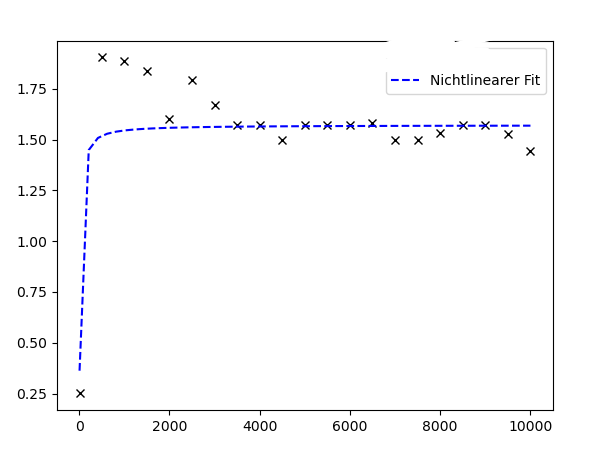
\includegraphics[width=\textwidth]{build/plot1.pdf}
    \caption{Messwerte und Theoriekurve der frequenzabhängigen Brückenspannung.} 
    \label{fig:plot1}
\end{figure}
\begin{flushleft}
Zusätzlich kann hier noch der Klirrfaktor berechnet werden. Dazu ist es allerdings notwendig die Berechnungen des Klirrfaktors $k$ nach Gleichung \eqref{eqn:GlasGoesklirr} anzunähern. 
Die Summe über alle Oberwellen wird hier durch die zweite Oberwelle nach unten abgeschätzt und es folgt
\end{flushleft}
\begin{equation*}
k = \frac{U_{2}}{U_{1}}
\end{equation*}
wobei $U_{1}$ die Amplitude der Grundwelle ist. Für die zweite Oberwelle $U_{2}$ mit $\Omega = 2$ gilt nach Formel \eqref{eqn:ya}.
\begin{equation*}
U_{2} = \frac{U_{B\text{,}{f_{0}}  }}{\sqrt{\frac{(\Omega^2 - 1)^{2}}{9(1- \Omega^2)^{2} + 9 \Omega^2}}} 
\end{equation*}
Die Spannung $U_{B\text{,}{f_{0}}}$ kann als die niedrigste gemessene Spannung aus Tabelle \ref{tab:frequencyitis} abgelesen werden. Es gilt somit.

\begin{equation*}
    U_{2} = \SI{0.001}{\volt} \cdot \sqrt{45} = \SI{6.71e-3}{\volt}
\end{equation*}
Da die Amplitude der Grundwelle $U_{1}$ für diese Messreihe $\SI{1}{\volt}$ beträgt, folgt ein Klirrfaktor von.
\begin{equation}
k = \SI{6.71e-3}{}
\end{equation}